\documentclass[11pt,reqno]{amsart}

\usepackage[margin=1.02in]{geometry}
\usepackage{amsmath,amssymb,amsthm,mathtools}
\usepackage{booktabs,array}
\usepackage{graphicx}
\usepackage{xcolor}
\usepackage{hyperref}
\raggedbottom
\emergencystretch=1.5em

\definecolor{navy}{HTML}{0F172A}
\definecolor{accent}{HTML}{1D4ED8}
\hypersetup{
  colorlinks=true,
  linkcolor=accent,
  citecolor=accent,
  urlcolor=accent,
  pdftitle={Finite-Memory Mirages, Unilateral Memory Cliffs, and Partial Common Funds in Zero-Communication Automata Games}
}

\newtheorem{theorem}{Theorem}[section]
\newtheorem{proposition}[theorem]{Proposition}
\newtheorem{lemma}[theorem]{Lemma}
\newtheorem{corollary}[theorem]{Corollary}
\theoremstyle{definition}
\newtheorem{definition}[theorem]{Definition}
\theoremstyle{remark}
\newtheorem{remark}[theorem]{Remark}

\newcommand{\R}{\mathbb{R}}
\newcommand{\Z}{\mathbb{Z}}
\newcommand{\N}{\mathbb{N}}
\newcommand{\E}{\mathbb{E}}
\newcommand{\Prob}{\mathbb{P}}
\newcommand{\one}{\mathbf{1}}
\DeclareMathOperator{\osc}{osc}

\title[Finite-Memory Mirages and Partial Common Funds]{Finite-Memory Mirages, Unilateral Memory Cliffs,\\
and Partial Common Funds in Zero-Communication\\
Automata Games}

\author{Project ReMath}
\date{November 24, 2026}
\subjclass[2020]{Primary 60J10, 91A22, 91A20; Secondary 60F10, 68Q45}
\keywords{Tsetlin automata, memory-depth paradox, Stag Hunt, Common Fund, Obshchaya kassa, threshold public good, Nash equilibrium, period-three limit cycle, large-population mean field}

\begin{document}

\begin{abstract}
In M.~L.~Tsetlin's Soviet school of collective automata games (1961--1966), while Tsetlin identified optimal finite memory in exogenously switching single-agent media, deep memory ($n \to \infty$) in stationary games was prized for asymptotic optimality, and payoff sharing was studied through Gelfand--Pyatetskii-Shapiro--Tsetlin's (1963) and Ginzburg--Krylov--Tsetlin's (1964) full $100\%$ \emph{Common Fund} (\emph{Obshchaya kassa}). In this companion to \cite{Paper1}, we establish three sharp finite-memory and partial-pooling phenomena proving that \emph{adding memory can catastrophically destroy collective welfare}, while \emph{partial pooling strictly below Nash equilibrium can achieve the exact social optimum---only to shatter the instant individual memory increases from $n=1$ to $n=2$}.

First, we analyze unilateral memory incentives in linear Tsetlin automata $L_{2n,2}$. Under matched homogeneous shocks ($\kappa_R=\kappa_P=1$), increasing one player's memory by \emph{one additional depth per action} (from 80 to 82 internal states: $(40,40)\to(41,40)$) in $(0.55,0.40,0.99,0.39)$ raises the upgrader's payoff from $0.549976$ to $0.670406$ while crashing mutual cooperation from $99.9837\%$ to $0.0018\%$. In $(0.52,0.45,0.999,0.44)$, for \emph{every} $n \ge 40$, at least one of $(n,n)$ and $(n+1,n+1)$ admits a strictly profitable one-depth deviation. In an $N$-player ($N \ge 3$) action-group-shared linear public good, sending one player's memory $m \to \infty$ followed by $n \to \infty$ causes a razor-sharp collapse of the $N-1$ peers at $d_* = h\frac{N-2}{N-1}$ (limiting peer cooperation equals $1, 1/2, 0$ below, at, and above $d_*$, with unanimous defection $\to 1$ above $d_*$).

Second, for the equal-memory independent constant-hare Stag Hunt ($0<S<P=T<R<1$, $P>1/2$), we prove $U_n = \frac{\pi_n(CC)}{1-\pi_n(CC)} \asymp G_n \lambda^n$ ($G_n = \sum_{j=0}^{n-1}(S/(1-S))^j$, $\lambda = \rho_P^2/\rho_R$), with exact leading constant $K(R,P,S) = \frac{(2P-1)^2}{(1-S)(2R-1)}$ for $1/2 \le S < P$ via an infinite-ladder transmission cancellation $(1-\rho_P)h_C = (1-\rho_R)(1-h_D)$. Using monotone coupling and exact rational witnesses, we certify \emph{open parameter regions strictly on both sides of $S=1/2$} where cooperation starts below $37.5\%$ at $n=1$, surges above $80\%$ at moderate memory ($n=10$ to $30$), and collapses to $0\%$ as $n\to\infty$. Along any subcritical sequence $(S_j,R_j) \to (1/2, R_*)$ with $\delta_j = -\log\lambda(R_j) > 0$ and $b_j = \log(S_j/(1-S_j))/\delta_j \to b < 1$, the rescaled odds collapse onto $g_b(x) = e^{-x}\int_0^x e^{bt}\,dt$, driving $\max_n \pi_n(CC) \to 1$ from \emph{either side} of $S=1/2$ while $\lim_{n\to\infty}\pi_n(CC)=0$ for all sufficiently large $j$.

Third, we introduce \emph{partial} Common Funds ($\alpha \in [0,1]$) in $N$-player threshold public goods with quorum $\theta \in (0,1/2)$ and cost $c$. At depth $n=1$ ($L_{2,2}$ or $B_{2,2}$), we prove a general parametric theorem identifying the unique limiting welfare-maximizing share $A_1 = \frac{c\theta-(1-H)(1-2\theta)}{2c\theta(1-\theta)} \in [0,1)$, attaining the social optimum $H-c\theta$ with finite-$N$ shift $\alpha_N^{\mathrm{opt}}-A_1 = \Theta(\sqrt{\log N/N})$ and optimal deficit $\Theta(\sqrt{\log N/N})$ (vs.\ $\Theta(1/\log N)$ at fixed $A_1$). On the benchmark $(0.80,0.97,0.60,1/4)$, blind depth-$1$ agents attain $0.82$ at $A_1 = 3/5$---strictly below the limiting pivotal Nash share $\alpha_{\mathrm{Nash}} = 43/60$, beating both private ($0.68$) and full pooling ($0.67$). For arbitrary depth $n \ge 1$ ($N\to\infty$ first), the feasible quota-balance shares $A_n$ increase strictly and cross $\alpha_{\mathrm{Nash}}$ at the \emph{exact critical cutoff $n_c = 2$}: $A_1 = 3/5 < 43/60 < A_2 = (11-4\sqrt{3})/5 \approx 0.8144 < A_3 \approx 0.8863$. For every $n \ge 2$ and $\alpha \le 43/60$, no productive fixed point exists and a positive welfare gap persists uniformly in $N$ (with locally attracting period-$3$ limit cycles at $n=2, \alpha=0.70$), while $1 - A_n \sim \frac{p_*(1-p_*)}{cn}\log\frac{1-\theta}{\theta}$. Core algebraic identities, depth-$1$ rational certificates, and the $n_c=2$ cutoff are verified in standalone Lean~4.
\end{abstract}

\maketitle

\section{Introduction}

In the classical works of M.~L.~Tsetlin \cite{Tsetlin1961,Tsetlin1963}, I.~M.~Gelfand, I.~I.~Pyatetskii-Shapiro, and M.~L.~Tsetlin \cite{GPST1963}, S.~L.~Ginzburg, V.~Yu.~Krylov, and M.~L.~Tsetlin \cite{GKT1964}, B.~G.~Pittel \cite{Pittel1965}, and V.~I.~Krinskii \cite{Krinskii1966}, finite-memory learning automata were celebrated for two structural mechanisms:
\begin{enumerate}
  \item \emph{Asymptotic optimality via deep memory}: Whereas Tsetlin \cite{Tsetlin1963} already discovered an optimal finite memory depth for a single automaton tracking an \emph{exogenously switching} random medium, in stationary games taking $n \to \infty$ was traditionally studied as the mechanism that suppresses switching noise and selects high-payoff profiles.
  \item \emph{The Common Fund (\emph{Obshchaya kassa})}: Introduced by Gelfand, Pyatetskii-Shapiro, and Tsetlin \cite{GPST1963} and tested in placement games by Ginzburg, Krylov, and Tsetlin \cite{GKT1964}, pooling $100\%$ of all players' payoffs ($\alpha = 1$) converts a non-cooperative game into a team game.
\end{enumerate}

The present paper demonstrates that in stationary strategic games, both paradigms exhibit sharp quantitative reversals once one studies \emph{unilateral memory-depth deviations}, \emph{endogenous finite-memory non-monotonicity}, and \emph{partial income pooling ($\alpha \in (0,1)$)} across arbitrary depths $n \ge 1$. Together with our companion study \cite{Paper1} on correlated feedback and 2D escape geometry, we prove three core theorems:
\begin{itemize}
  \item \textbf{Unilateral Memory Cliffs (Section~\ref{sec:memory})}: Even when equal-memory societies converge to $100\%$ cooperation, expanding one player's memory by \emph{one additional depth per action} ($40 \to 41$, i.e.\ $80 \to 82$ internal states) raises that player's payoff by $+0.12$ while crashing mutual cooperation from $99.98\%$ to $0.0018\%$. In an explicit Prisoner's Dilemma, no adjacent equal-memory pair $\{(n,n),(n+1,n+1)\}$ ($n \ge 40$) resists one-depth deviations; and in an $N$-player action-group-shared linear public good ($N \ge 3$), one growing memory triggers a sharp peer collapse at $d_* = h\frac{N-2}{N-1}$.
  \item \textbf{Endogenous Finite-Memory Stag-Hunt Mirages (Section~\ref{sec:staghunt})}: In an equal-memory independent constant-hare Stag Hunt, cooperation rises from $<37.5\%$ at $n=1$ to $>80\%$ (and arbitrarily close to $100\%$) at moderate memory before collapsing to $0\%$ as $n \to \infty$ across certified \emph{open parameter regions strictly on both sides of $S=1/2$}, unified by an exact two-parameter universal scaling law $g_b(x) = e^{-x}\int_0^x e^{bt}\,dt$.
  \item \textbf{Partial Common Funds Below Nash and the Exact $n_c = 2$ Cutoff (Section~\ref{sec:fund})}: In $N$-player no-refund threshold public goods \cite{PalfreyRosenthal1984}, \emph{full} $100\%$ pooling fails (inducing $50\%$ wasteful volunteering, worse than $0\%$ private rewards). Yet at depth $n=1$, a \emph{partial} Common Fund strictly below the limiting pivotal Nash share achieves the exact social optimum $H - c\theta$ (with sharp finite-$N$ scaling $\Theta(\sqrt{\log N/N})$). Increasing individual memory from $n=1$ to $n=2$ immediately shatters this below-Nash advantage ($n_c = 2$): for every $n \ge 2$ and $\alpha \le \alpha_{\mathrm{Nash}}$, no productive fixed point exists, a positive stationary welfare gap persists uniformly in $N$, certified locally attracting period-$3$ limit cycles appear at $(n=2, \alpha=0.70)$, and the quota-balance shares approach $100\%$ at rate $1 - A_n \sim \frac{p_*(1-p_*)}{c n}\log\frac{1-\theta}{\theta}$.
\end{itemize}

\section{Unilateral Memory Cliffs and Strategic Instability}\label{sec:memory}

We consider linear Tsetlin automata $L_{2m,2}$ with $m$ memory depths per action ($0$ shallowest to $m-1$ deepest), where a reward deepens the current action by $1$ (capped at $m-1$) and a penalty reduces depth by $1$ (switching action at depth $0$). For a single automaton facing fixed reward probabilities $(x,y)$ on actions $(C,D)$, birth--death balance gives cooperation probability
\begin{equation}\label{eq:one-player-F}
  H_n(x) := \frac{1}{1-x}\sum_{j=0}^{n-1}\left(\frac{x}{1-x}\right)^j, \qquad
  F_n(x,y) := \frac{H_n(x)}{H_n(x) + H_n(y)}.
\end{equation}

\subsection{One Growing Player Against a Finite Population}
Fix all opponents' memory depths, letting $e$ encode their finite joint state. Assume the tagged player's reward and penalty probabilities are bounded below by $\varepsilon > 0$ everywhere, and that freezing the tagged player's action at $a \in \{C,D\}$ yields an irreducible opponent Markov chain $P_a$ with stationary law $\nu_a$, frozen tagged win mean $w_a := \nu_a p_a$, and frozen drift $u_a := 2w_a - 1$.

\begin{proposition}[Frozen-Environment Limit and Perron Selection]\label{prop:one-growing}
As the tagged player's memory $m \to \infty$ with opponent memories fixed:
\begin{enumerate}
  \item If $u_D > 0 > u_C$, the tagged player's stationary frequency in $D$ tends to $1$, the opponent state law tends to $\nu_D$, and the tagged player's expected payoff tends to $w_D$ (and symmetrically if $u_C > 0 > u_D$).
  \item If $\max(u_C, u_D) > 0$, the stationary action-switch rate vanishes and every subsequential limit of the joint law on $(a,e)$ has the form $t\,\delta_C \nu_C + (1-t)\,\delta_D \nu_D$.
  \item If $u_C < 0$ and $u_D < 0$, then $\limsup_{m\to\infty} W_1(m) \le 1/2$.
  \item If $u_C > 0$ and $u_D > 0$, let $P_a = B_a^+ + B_a^-$ split transitions by tagged reward/penalty and let $\theta_a > 0$ be the unique positive root of $\rho(e^{-\theta_a} B_a^+ + e^{\theta_a} B_a^-) = 1$. Whenever $\theta_D > \theta_C$ (resp.\ $\theta_C > \theta_D$), action $D$ (resp.\ $C$) is selected with probability tending to $1$.
\end{enumerate}
\end{proposition}

\begin{proof}[Proof outline]
Solving the finite Poisson equation $(I - P_a)g = 2p_a - 1 - u_a$ bounds the capped visit duration uniformly by $(1 + \osc g)/|u_a|$ when $u_a < 0$. When $u_a > 0$, the uncapped ergodic theorem guarantees probability $\ge \varepsilon^H/2$ of reaching cap $m-1$, forcing expected duration $\Omega(m)$ (and $\Theta(e^{\theta_a m})$ via the Perron martingale $e^{-\theta_a d} v(e)$). Equal stationary entry fluxes into $C$ and $D$ select the action of larger growth order, while $\|\eta_a P_a - \eta_a\|_1$ is bounded by the vanishing switch rate. For $u_C, u_D < 0$, exact stationary depth balance $2W_1 - 1 = \E[p_a(e)\one_{\{d=m-1\}}] - \E[(1-p_a(e))\one_{\{d=0\}}]$ with vanishing cap occupancy yields $\limsup W_1 \le 1/2$.
\end{proof}

\subsection{The \texorpdfstring{$+1$}{+1}-Depth Apocalypse, Adjacent-Pair Instability, and \texorpdfstring{$N$}{N}-Player Public-Good Cliff}

\begin{theorem}[Memory-Incentive Cliffs]\label{thm:memory-cliffs}
Consider linear Tsetlin automata $L_{2n,2}$.
\begin{enumerate}
  \item \textbf{The $+1$-Depth Apocalypse.} Consider the strict Prisoner's Dilemma with $(R, P, T, S) = (0.55, 0.40, 0.99, 0.39)$, matched homogeneous shocks ($\kappa_R = \kappa_P = 1$), and independent mixed outcomes. Equal-memory pairs synchronize on a single recurrent class with $\pi_{n,n}(CC) = F_n(R,P) \to 1$ and $W_1(n,n) \to 11/20 = 0.55$, whereas sending $m \to \infty$ followed by $n \to \infty$ yields $W_1(m,n) \to 143/210 \approx 0.68095$. Already at $n = 40$, adding one depth per action (80 to 82 internal states) yields exact rational Poisson-residual enclosures:
  \[
    W_1(40,40) \in (0.5499755023,\, 0.5499755025), \qquad
    W_1(41,40) \in (0.6704057221,\, 0.6704057224),
  \]
  while mutual cooperation crashes from $\pi_{40,40}(CC) = 99.9837\%$ to $\pi_{41,40}(CC) = 0.0018\%$. (Conversely, in the Chicken game $(0.70, 0.20, 0.71, 0.23)$ under the same feedback rule, equal memories give $W_1(n,n)\to 0.70$, whereas $\limsup_{m\to\infty} W_1(m,n) \le 0.50$ for all large $n$, and upgrading $(10,10)\to(11,10)$ strictly loses: $0.69993 \to 0.69800$.)

  \item \textbf{All-Large Adjacent-Pair Instability.} In the strict Prisoner's Dilemma $(R,P,T,S) = (0.52, 0.45, 0.999, 0.44)$ with matched homogeneous outcomes and independent mixed outcomes, equal memories select mutual cooperation ($\pi_{n,n}(CC) \to 1$), yet for \emph{every integer $n \ge 40$}, at least one of $(n,n)$ and $(n+1,n+1)$ admits a strictly profitable one-depth unilateral deviation.

  \item \textbf{Sharp $N$-Player Public-Good Memory-Asymmetry Cliff.} For $N \ge 3$, consider the symmetric linear public good with individual win probability
  \[
    p_i = b + h\frac{k_{-i}}{N-1} + d\,\one_{\{i \text{ defects}\}}, \qquad 0 < d < h,
  \]
  where $k_{-i}$ counts cooperating opponents, $R = b+h$, $P = b+d$, $T = b+h+d$, and $0 < b < 1/2 < P$, $R - h/(N-1) > 1/2$, $T < 1$, with action-group-shared uniform feedback (independent across the $C$ and $D$ groups). Give one player memory $m$ and the other $N-1$ players memory $n$, and let $G_{m,n}$ be the stationary probability that all $N-1$ ordinary players cooperate. Set $d_* := h\frac{N-2}{N-1}$. Whereas equal memories ($m=n$) yield $\Pr(\text{all }C) = F_n(R,P) \to 1$ for all $d < h$, expanding a single player's memory causes a sharp transition:
  \begin{equation}\label{eq:n-player-cliff}
    \lim_{n\to\infty}\limsup_{m\to\infty}\bigl|G_{m,n} - g(d)\bigr| = 0, \qquad
    g(d) :=
    \begin{cases}
      1, & d < d_*,\\
      1/2, & d = d_*,\\
      0, & d > d_* \quad (\text{unanimous defection} \to 1).
    \end{cases}
  \end{equation}
\end{enumerate}
\end{theorem}

\begin{proof}[Proof outline]
For Part (1), Proposition~\ref{prop:one-growing}(1) yields frozen payoffs $w_C \to 0.39 < 1/2 < 0.40 + 0.59\cdot\frac{10}{21} = 143/210 = \lim w_D$. The finite payoff enclosures are certified by exact rational evaluation of $r + P v - v$ separately on the $80$-state synchronized recurrent class at $(40,40)$ (enclosure width $4.0 \times 10^{-70}$) and on the $6{,}560$-state recurrent class at $(41,40)$ (enclosure width $1.76 \times 10^{-66}$, \texttt{experiments/phase1\_memory.py}).

For Part (2), at any equal pair $(k,k)$ the synchronized chain places positive mass on $DD$, so $W_1(k,k) < R$. At depths $(n+1, n)$, write $M = \{CD, DC\}$; then
\[
  W_1 + W_2 - 2R = (T + S - 2R)\pi_M - 2(R - P)\pi_{DD}.
\]
Decompose into alternating homogeneous blocks (no mixed profile) and mixed blocks. Whenever a $DD$ run is entered, the smaller defection depth is $0$, so stopping the drift inequality bounds its mean duration by $g = 1/(1-2P)$. Entering a homogeneous block at equal depth $0$ places every direct $DD\to CC$ jump at equal \emph{cooperative} depth $0$, from which gambler's ruin gives probability $\ge c = 1 - (1-R)/R$ of separation at cap $n-1$ before any subsequent $DD$ (once separated, the deeper player keeps its $+1$ lead until a mixed round), bounding expected $DD$ visits by $g/c$. Entering from mixed play at distinct depths yields expected $DD$ visits $\le g H_n$ with $H_n = \max(1+B_n/c, A_n/c)$, where $A_n = ((1-R)/R)^n$ and $B_n = (P/(1-P))^{n-1}$. Entering equal depth $0$ from mixed play requires a double loss (rate $\le (1-S)(1-T)\pi_M$), and for $n \ge K = 15$ a mixed block has mean duration $\ge L := \sum_{j=0}^{K-1}(v_j - j(1-T)) > 4.092$ (computed via exact rational recursion for the uncapped $S$-survival probability $v_j$). Thus
\[
  \frac{\pi_{DD}}{\pi_M} \le g\Bigl(\frac{H_n}{L} + \frac{(1-S)(1-T)}{c}\Bigr),
\]
which is nonincreasing in $n$ and gives $W_1 + W_2 - 2R > 0.0449\,\pi_M > 0$ for all $n \ge 40$. Hence at least one player at $(n+1,n)$ strictly beats $R$, creating a profitable one-depth deviation from either $(n,n)$ or $(n+1,n+1)$.

For Part (3), action-group-shared feedback synchronizes the $N-1$ equal-memory players on the unique recurrent class. Given a frozen tagged action $C$ or $D$, the synchronized group behaves as a single $L_{2n,2}$ automaton with cooperation probabilities $f_C = F_n(R,\, P + h/(N-1))$ and $f_D = F_n(R - h/(N-1),\, P)$, in both of which the advantage of cooperation is $R - P - h/(N-1) = d_* - d$. Hence $f_C, f_D \to g(d)$ as $n\to\infty$. Since $w_D = P + (T-P)f_D \ge P > 1/2$, Proposition~\ref{prop:one-growing}(2) pins every $m\to\infty$ limit of $G_{m,n}$ between $f_C$ and $f_D$; for $d > d_*$, eventually $w_C = b + (R-b)f_C < 1/2 < w_D$, so Proposition~\ref{prop:one-growing}(1) drives the tagged player to $D$ and the group to unanimous defection ($\to 1$).
\end{proof}

\begin{figure}[t]
  \centering
  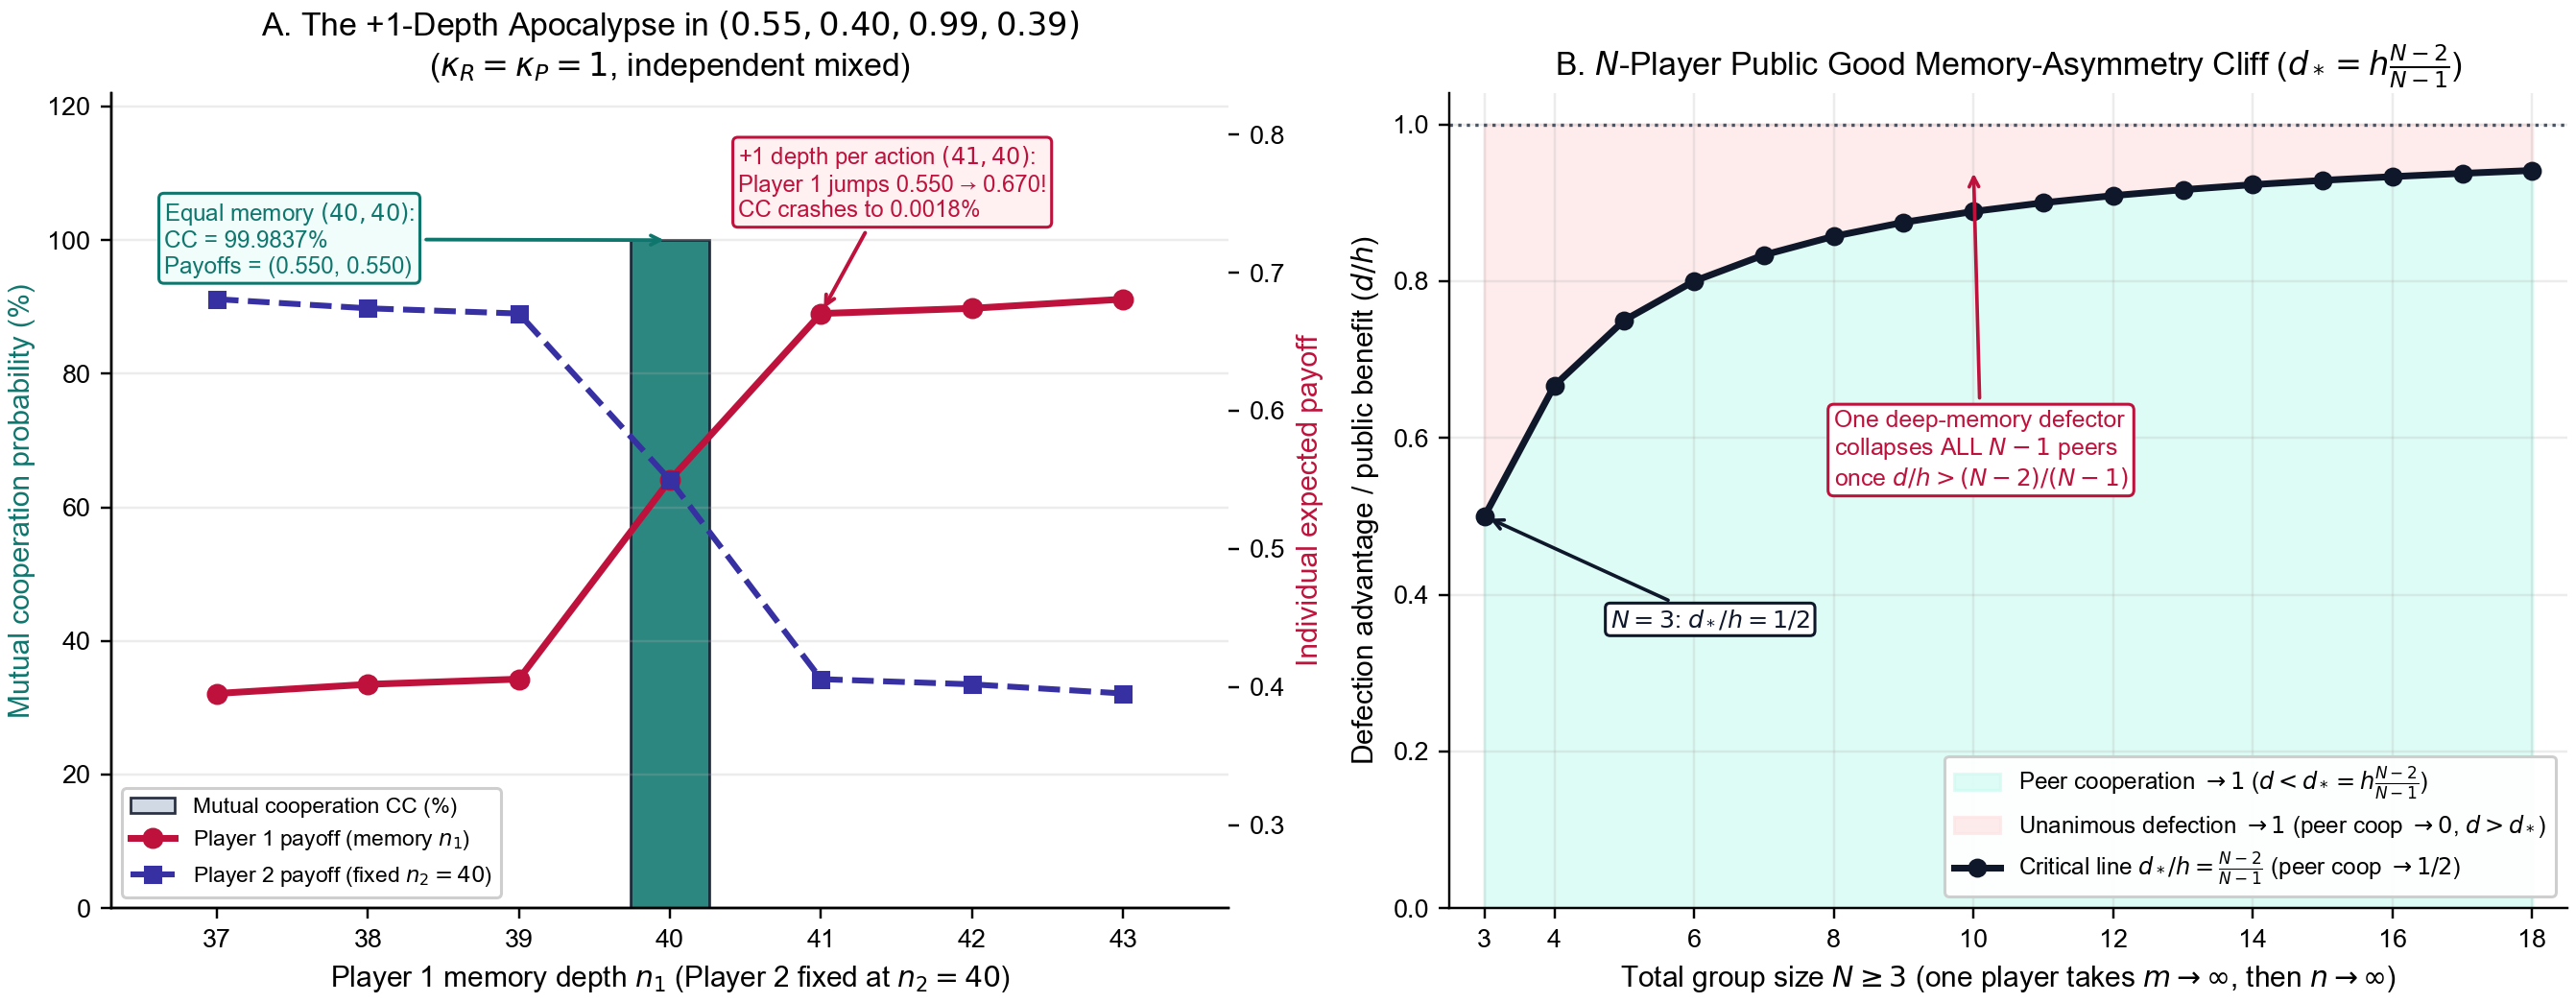
\includegraphics[width=\textwidth]{figs/p2_fig1_memory_cliffs.png}
  \caption{\textbf{Unilateral memory-incentive cliffs.}
  \textbf{(A)} 80-digit GTH stationary sweep $(n_1, 40)$ in $(0.55,0.40,0.99,0.39)$ ($\kappa_R=\kappa_P=1$): mutual cooperation forms a sharp peak ($99.9837\%$) strictly at $n_1 = 40$, surrounded by $<0.003\%$ wasteland, while adding one depth per action ($40 \to 41$) boosts Player~1's payoff from $0.550$ to $0.670$.
  \textbf{(B)} Exact $N$-player action-group-shared public-good phase boundary $d_*/h = (N-2)/(N-1)$ separating peer cooperation ($\to 1$ for $d < d_*$) from unanimous defection ($\to 1$, peer cooperation $\to 0$, for $d > d_*$) when one agent expands memory ($m \to \infty$, then $n \to \infty$).}
  \label{fig:p2-cliffs}
\end{figure}

\section{Endogenous Stag-Hunt Mirages on Both Sides of \texorpdfstring{$S=1/2$}{S=1/2}}\label{sec:staghunt}

Consider two equal-memory linear Tsetlin automata $L_{2n,2}$ playing an independent constant-hare Stag Hunt: mutual stag ($CC$) pays win probability $R$, solo stag ($CD, DC$) pays $S$, and hare always pays $P = T$, with
\begin{equation}\label{eq:stag-order}
  0 < S < P = T < R < 1, \qquad P > 1/2.
\end{equation}
Set $p_n := \pi_n(CC)$, $U_n := \frac{p_n}{1-p_n}$, $\rho_x := \frac{1-x}{x}$, $a := \frac{S}{1-S}$, $\lambda := \frac{\rho_P^2}{\rho_R}$, and
\begin{equation}\label{eq:stag-defs}
  G_n := \sum_{j=0}^{n-1} a^j, \qquad
  K(R,P,S) := \frac{(2P-1)^2}{(1-S)(2R-1)}, \qquad
  R_c(P,S) := \frac{P^2}{P^2 + (1-P)^2 \max(1, a)}.
\end{equation}

\begin{theorem}[Stag-Hunt Odds Scaling, Open-Region Mirages, and Universal Collapse]\label{thm:staghunt}
Assume \eqref{eq:stag-order}.
\begin{enumerate}
  \item \textbf{Two-Sided Odds Bounds and Exact Constant.} There exist constants $0 < c < C < \infty$ (uniform on compact subintervals of $R \in (P,1)$ at fixed $P,S$) such that
  \begin{equation}\label{eq:stag-bounds}
    c\, G_n \lambda^n \le U_n \le C\, G_n \lambda^n \qquad \text{for all } n \ge 1.
  \end{equation}
  Hence $p_n \to 0$ for $R < R_c(P,S)$ and $p_n \to 1$ for $R > R_c(P,S)$. Moreover, for every $1/2 \le S < P$,
  \begin{equation}\label{eq:stag-asymp}
    U_n \sim K(R,P,S)\, G_n \lambda^n \qquad (n \to \infty),
  \end{equation}
  giving at criticality $R = R_c(P,S)$: $1 - p_n \sim 1/(K n)$ when $S = 1/2$, and $p_n \to K/(K + a - 1)$ when $S > 1/2$.

  \item \textbf{Monotone Coupling and Certified Open-Region Mirages on Both Sides of $S=1/2$.} Whenever $1-P \le S \le R$, $p_n(R,P,S)$ is nondecreasing in $(R,S)$ at fixed $(P,n)$. Fixing $P = T = 4/5$, throughout each of the three open curved-boundary regions:
  \begin{itemize}
    \item $\mathcal{R}_1$: $0.47 < S < 1/2$, $0.94 < R < 16/17$ ($m = 16$, $p_1 \le 3757/10042 < 3/8$);
    \item $\mathcal{R}_2$: $0.52 < S < 208/395$, $0.935 < R < R_c(4/5,S)$ ($m = 10$, $p_1 \le 220211/597796 < 3/8$);
    \item $\mathcal{R}_3$: $0.5499 < S < 1136/2065$, $0.929 < R < R_c(4/5,S)$ ($m = 18$, $p_1 \le \frac{9854063369}{27894660164} < \frac{3}{8}$);
  \end{itemize}
  every game satisfies $p_1 < 37.5\%$, $\max_n p_n \ge p_m > 80\%$, and $\lim_{n\to\infty} p_n = 0$.

  \item \textbf{Two-Parameter Universal Scaling Law.} Fix $P \in (1/2, 1)$, let $R_* := R_c(P,1/2) = \frac{P^2}{P^2+(1-P)^2}$ and $K_* := K(R_*,P,1/2)$. Along any sequence $(S_j, R_j) \to (1/2, R_*)$ with $\delta_j := -\log\lambda(R_j) > 0$ and $b_j := \frac{\log(S_j/(1-S_j))}{\delta_j} \to b < 1$, whenever $\delta_j n_j \to x \in (0,\infty)$,
  \begin{equation}\label{eq:gb-law}
    \frac{\delta_j U_{j,n_j}}{K_*} \longrightarrow g_b(x) := e^{-x}\int_0^x e^{bt}\,dt =
    \begin{cases}
      \dfrac{e^{-(1-b)x} - e^{-x}}{b}, & b \neq 0,\\[6pt]
      x e^{-x}, & b = 0.
    \end{cases}
  \end{equation}
  For all sufficiently large $j$, the game is subcritical ($\lim_{n\to\infty} p_{j,n} = 0$) and every maximizing finite depth $m_j$ satisfies $\delta_j m_j \to x_b$ ($x_0 = 1$, $x_b = -\frac{\log(1-b)}{b}$ for $b \neq 0$) and $1 - \max_n p_{j,n} \sim \frac{\delta_j}{K_* g_b(x_b)} \to 0$, proving that peaks approach $100\%$ from \emph{either side} of $S = 1/2$.
\end{enumerate}
\end{theorem}

\begin{proof}[Proof outline]
Replace transitions inside $A := CC$ by solo-stag probability $S$ to obtain a reversible product reference chain outside $A$ whose exact one-player stationary weights are $m(D_d) = \rho_P^{n-1-d}$ and $m(C_d) = \frac{P\rho_P^n}{1-S} a^d$ ($0 \le d < n$, $Z = \sum m$). With one-player $D\to C$ flux $f = P\rho_P^n / Z$ and $u = f G_n / (1-S)$, independence gives the exact stationary entry flux into $A$:
\begin{equation}\label{eq:ref-flux}
  F = u^2 - (u - f)^2 = f^2\Bigl(\frac{2G_n}{1-S} - 1\Bigr) \asymp G_n \rho_P^{2n}.
\end{equation}
Comparing excursions between deepest hare $z = (D_*,D_*)$ and deepest stag $w = (C_*,C_*)$ yields $U_n \asymp G_n \lambda^n$. For $1/2 \le S < P$ (and uniformly along $S_n \to 1/2$), entry into $A$ occurs overwhelmingly at a boundary site $(C_0, C_k)$ with $k \to \infty$. On the infinite half-ladder, let $h_C$ be the probability of reaching deep $CC$ starting at $(C_0, C_\infty)$, and let $h_D$ be the probability of reaching deep $CC$ starting immediately across the interface at $(D_0, C_\infty)$ (so $1 - h_D$ is the escape probability from $(D_0, C_\infty)$). Detailed balance across the single-step interface gives $h_D = \rho_P h_C$, which combined with the one-step recursion yields the exact transmission cancellation
\begin{equation}\label{eq:ladder-cancel}
  (1 - \rho_P) h_C = (1 - \rho_R)(1 - h_D),
\end{equation}
canceling boundary re-entry correlations and yielding $K(R,P,S) = \frac{(2P-1)^2}{(1-S)(2R-1)}$.

For Part (2), ordering each player's $2n$ levels from deepest hare to deepest stag makes the upward transition probability ($1-P$ on hare, $S$ on solo stag, $R$ on mutual stag) nondecreasing in both states and in $(R,S)$ whenever $1-P \le S \le R$. Coupling via shared independent uniforms preserves coordinatewise order at all times, so $p_n$ is nondecreasing in $(R,S)$. Exact rational GTH solves at the three lower corners $(0.47,0.94,m=16)$, $(0.52,0.935,m=10)$, and $(0.5499,0.929,m=18)$ certify $p_m = 0.803242, 0.812763, 0.800865 > 4/5$, while the exact 4-state $n=1$ formula at the upper corners certifies $p_1 \le \text{bound} < 3/8$ across each entire open region (via 368 certified 76-digit solves in \texttt{phase2b\_staghunt\_robustness.py}). For Part (3), with $a_j = e^{b_j \delta_j}$ and $\lambda_j = e^{-\delta_j}$, $G_{n_j}\lambda_j^{n_j}$ equals $n_j e^{-\delta_j n_j}$ when $b_j = 0$ and $(e^{-(1-b_j)\delta_j n_j} - e^{-\delta_j n_j})/(e^{b_j\delta_j}-1)$ when $b_j \neq 0$; uniform excursion bounds (valid across $S_j \to 1/2$, see \texttt{phase2b\_staghunt\_robustness.md}) give $\delta_j U_{j,n_j}/K_* \to g_b(x)$, and the uniform two-sided envelope $\delta_j G_n \lambda_j^n \le x e^{-(1 - \max(0, b_j)) x}$ ($x = \delta_j n$, since $G_n \le n \max(1, a_j^n)$) vanishes as $x \to 0^+$ and $x \to \infty$ whenever $b < 1$, forcing $\delta_j m_j$ into a compact subinterval of $(0,\infty)$ and hence $\delta_j m_j \to x_b$.
\end{proof}

\begin{figure}[t]
  \centering
  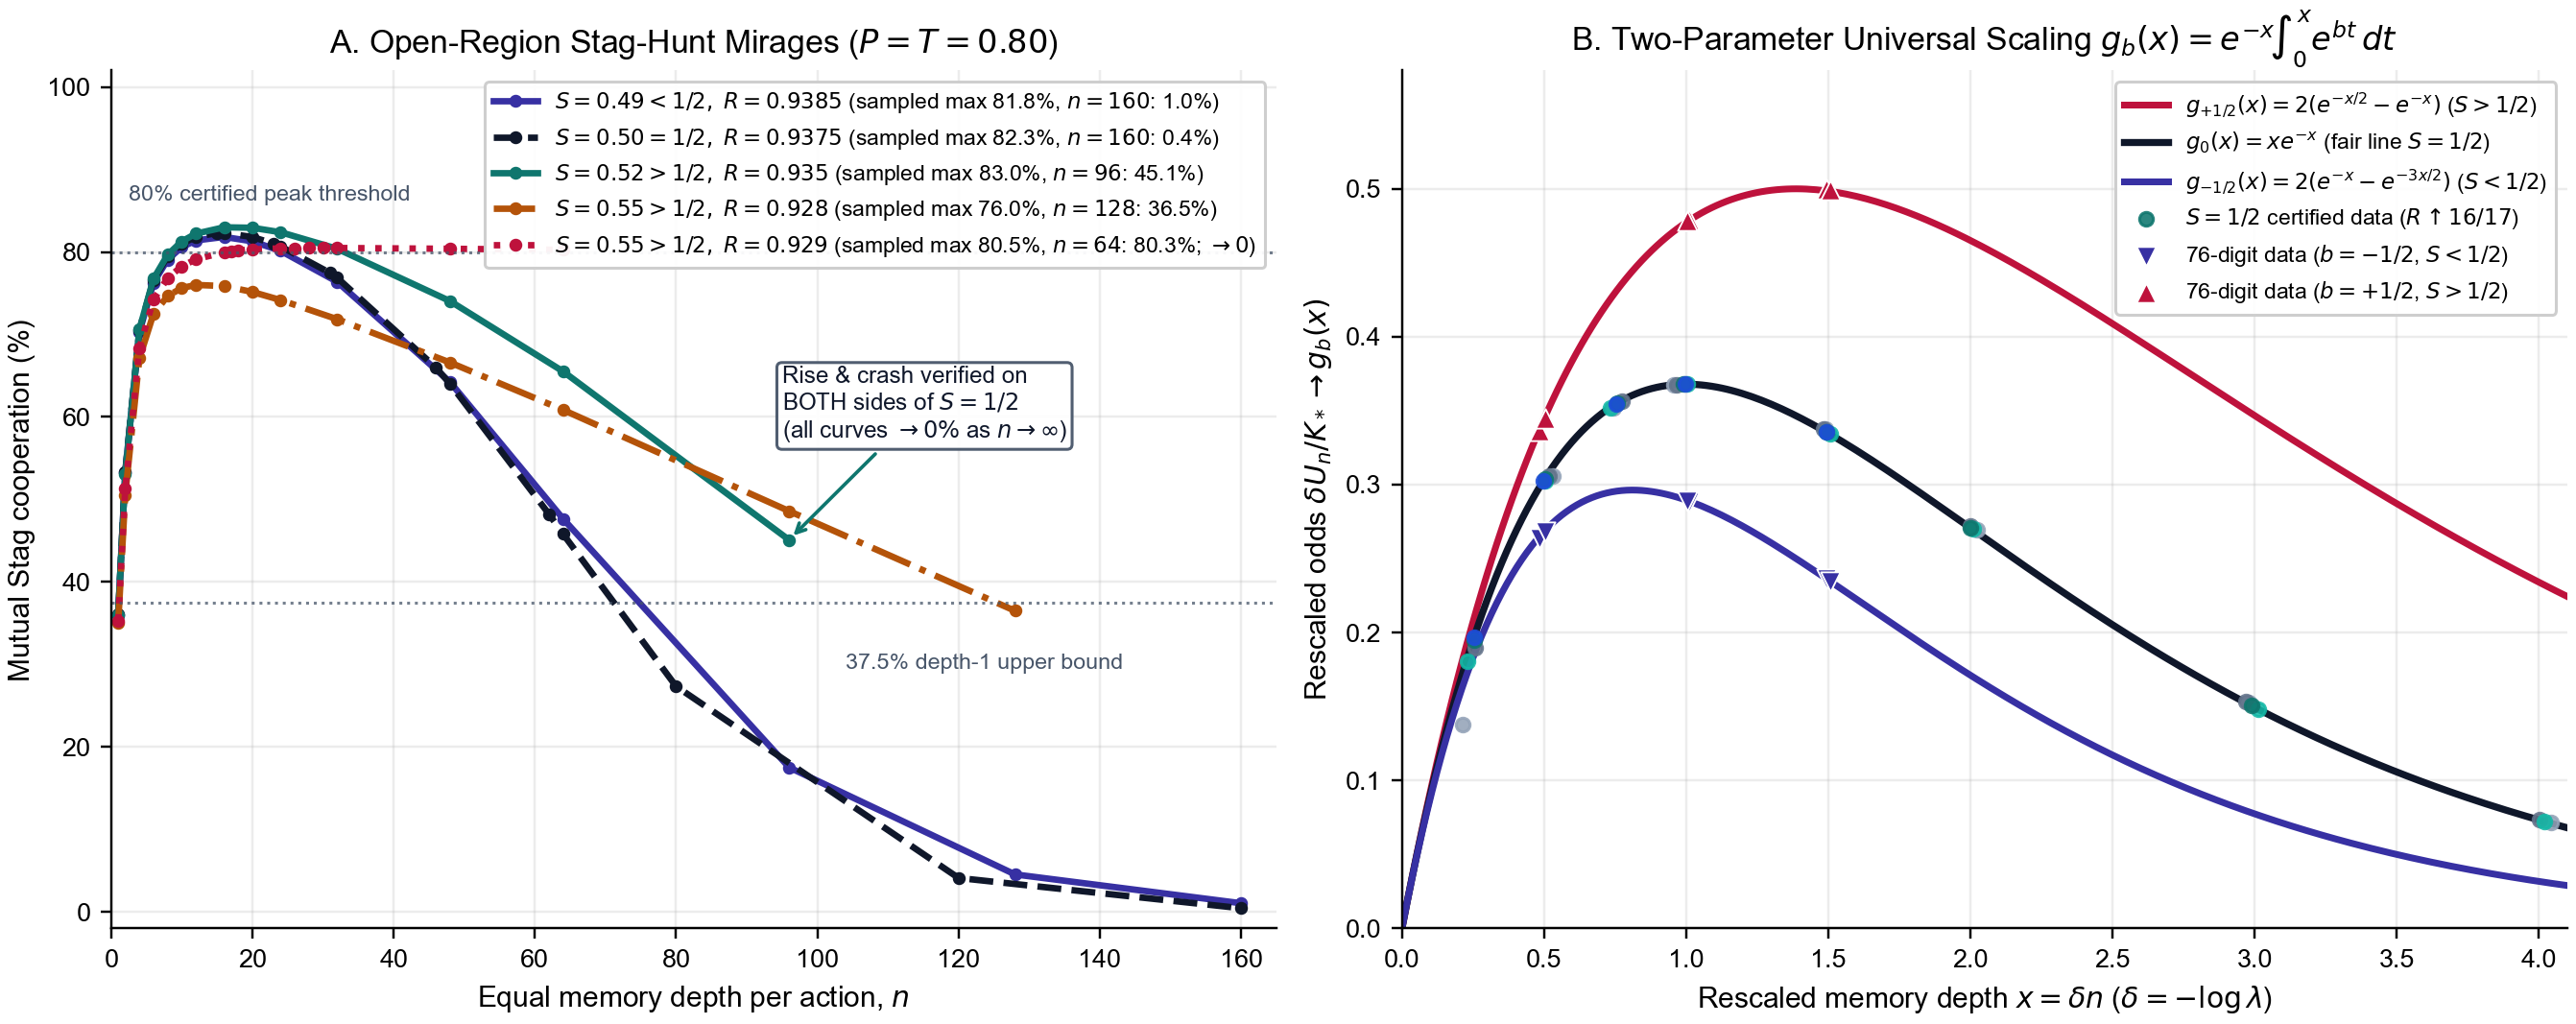
\includegraphics[width=\textwidth]{figs/p2_fig2_staghunt_mirages.png}
  \caption{\textbf{Open-region Stag-Hunt mirages on both sides of $S=1/2$ and universal $g_b(x)$ scaling.}
  \textbf{(A)} Certified 76-digit cooperation curves at $P = T = 0.80$ strictly below ($S=0.49$), at ($S=0.50$), and strictly above ($S=0.52, 0.55$) the fair line $S=1/2$: all curves start below $37.5\%$ at $n=1$, reach displayed sample peaks of approximately $76\%$--$83\%$, and satisfy $\lim_{n\to\infty} p_n = 0$ (visibly decaying on both sides of $S=1/2$, while the slow $S=0.55, R=0.929$ trace stays at $80.3\%$ at $n=64$ before its eventual exponential collapse).
  \textbf{(B)} Asymptotic collapse of 48 certified 76-digit observations across $b = -1/2, 0, +1/2$ toward the universal curve $g_b(x) = e^{-x}\int_0^x e^{bt}\,dt$.}
  \label{fig:p2-staghunt}
\end{figure}

\section{Partial Common Funds Below Nash and the Exact \texorpdfstring{$n_c=2$}{n\_c=2} Cutoff}\label{sec:fund}

In Gelfand--Pyatetskii-Shapiro--Tsetlin \cite{GPST1963} and Ginzburg--Krylov--Tsetlin \cite{GKT1964}, the \emph{Common Fund} (\emph{Obshchaya kassa}) pools $100\%$ of all $N$ players' rewards. We generalize this to an arbitrary \emph{partial} pooling fraction $\alpha \in [0,1]$ in a no-refund threshold public good \cite{PalfreyRosenthal1984} with quorum $\theta \in (0, 1/2)$, base probabilities $0 < c < L < H < 1$, and net productive optimum $M := H - c\theta > L$.

At each round, if fraction $x = k/N$ of the $N$ players contribute ($C$), the base success probability is $t(x) = L$ for $x < \theta$ and $t(x) = H$ for $x \ge \theta$. Contributors pay cost $c$ regardless of quorum, so raw payoffs are $p_C^{\mathrm{raw}} = t(x) - c$ and $p_D^{\mathrm{raw}} = t(x)$ with population mean $\bar p = t(x) - c x$. Under partial Common Fund pooling $\alpha \in [0,1]$, each player receives independent Bernoulli feedback with pooled win probability $(1-\alpha)p_i^{\mathrm{raw}} + \alpha \bar p$, i.e.,
\begin{equation}\label{eq:pooled-probs}
  p_D(x,\alpha) = t(x) - c\alpha x, \qquad
  p_C(x,\alpha) = p_D(x,\alpha) - c(1-\alpha).
\end{equation}
All $N$ players use identical synchronous automata of memory depth $n \ge 1$ per action ($L_{2n,2}$ with boundary switch probability $\nu = 1$, or $B_{2n,2}$ with $\nu = 1/2$). Let $W_{N,n}(\alpha) := \E_{\pi_{N,n}}[t(X) - c X]$ denote stationary mean welfare (capped globally by $M = H - c\theta$), and let $\rho_N(\alpha) := M - W_{N,1}(\alpha)$.

\subsection{Rational Benchmark versus Depth-1 Partial Common Fund}
For rational players (when $\lceil \theta N \rceil \ge 2$), all-defection is always a strict Nash equilibrium; an exactly-quorum pure profile is a Nash equilibrium for feasible $\alpha \in [0,1]$ if and only if a pivotal contributor's gain $H-L$ covers the unpooled cost $c[1-\alpha(1-1/N)]$, i.e.\
\[
  \alpha \in [0,1] \cap \bigl[\alpha_{\mathrm{Nash}}(N),\, \infty\bigr), \qquad
  \alpha_{\mathrm{Nash}}(N) := \frac{1 - (H-L)/c}{1 - 1/N} \longrightarrow \alpha_{\mathrm{Nash}} := 1 - \frac{H-L}{c}.
\]
(If $\alpha_{\mathrm{Nash}}(N) \le 0$, zero sharing already suffices; if $\alpha_{\mathrm{Nash}}(N) > 1$, no feasible share supports a quorum Nash profile.) When $\alpha_{\mathrm{Nash}} \in (0,1)$, for any $\alpha < \alpha_{\mathrm{Nash}}$ defection is strictly dominant for all large $N$ (with indifference at the limiting threshold $\alpha_{\mathrm{Nash}}$).

\begin{theorem}[General Parametric Depth-1 Partial Common Fund]\label{thm:fund-n1}
Fix $\theta \in (0, 1/2)$ and $0 < c < L < H < 1$ with $H - c\theta > L$, $\nu(1 - H + c) < 1 - \theta$, and
\begin{equation}\label{eq:A1-formula}
  A_1 := \frac{c\theta - (1-H)(1-2\theta)}{2c\theta(1-\theta)} \in [0, 1).
\end{equation}
For both $L_{2,2}$ ($\nu=1$) and $B_{2,2}$ ($\nu=1/2$) as $N \to \infty$:
\begin{enumerate}
  \item Every sequence of finite-$N$ welfare maximizers satisfies $\alpha_N^{\mathrm{opt}} \to A_1$ and $W_{N,1}(\alpha_N^{\mathrm{opt}}) \to M = H - c\theta$ (strictly beating full pooling $\alpha = 1$, where $x \to 1/2$ gives welfare $H - c/2 < M$, and strictly beating pure private play $\alpha = 0$ whenever $A_1 > 0$).
  \item Fixed-$A_1$ welfare suffers logarithmic deficit $\rho_N(A_1) = \Theta(1/\log N)$, whereas optimal tuning approaches $A_1$ from above with sharp scaling
  \begin{equation}\label{eq:finite-N-rate}
    \alpha_N^{\mathrm{opt}} - A_1 = \Theta\!\left(\sqrt{\frac{\log N}{N}}\right), \qquad
    \min_{\alpha \in [0,1]} \rho_N(\alpha) = \Theta\!\left(\sqrt{\frac{\log N}{N}}\right).
  \end{equation}
  \item Whenever $A_1 < 1 - (H-L)/c$, blind depth-$1$ automata attain the exact social optimum $M$ strictly inside the dominant-defection regime below Nash. In the one-quarter benchmark $(L,H,c,\theta) = (0.80, 0.97, 0.60, 1/4)$,
  \[
    A_1 = \frac{3}{5} = 0.60 < \frac{43}{60} = \alpha_{\mathrm{Nash}}, \qquad
    W_{N,1}(0) \to 0.68, \quad W_{N,1}(3/5) \to 0.82, \quad W_{N,1}(1) \to 0.67.
  \]
\end{enumerate}
\end{theorem}

\begin{proof}[Proof outline]
In branch $e = 1-t$, conditional mean next cooperation is $F_e(x) = x + \nu b_e(x)$ with $b_e(x) = e(1-2x) + c x(2\alpha - 1 - 2\alpha x)$. Each branch contracts globally around its unique root $x_e(\alpha) \in (0, 1/2]$, which crosses $\theta$ at $A_e = \frac{c\theta - e(1-2\theta)}{2c\theta(1-\theta)}$ ($A_{1-H} = A_1$). For $\alpha > A_1$, Hoeffding tails keep the chain exponentially trapped around $x_{1-H}(\alpha) \downarrow \theta$ as $\alpha \downarrow A_1$, yielding $\max_\alpha W_{N,1} \to M$. At fixed $\alpha = A_1$, a miss below $\theta$ bounces back via low-branch drift $\eta > 0$ and stays productive for $T = \Theta(\log N)$ steps, bounding failure probability $\pi_U$ by $O(1/\log N)$, matched by $\Omega(1/\log N)$ via global contraction to $O(N^{-1/2})$ and Berry--Esseen.

For \eqref{eq:finite-N-rate}, setting $\alpha = A_1 + t$ ($t > 0$ small) yields $\pi_U \le C e^{-2Nb^2 t^2}$ and $\rho_N(A_1+t) \le C[t + N^{-1/2} + e^{-2Nb^2 t^2}]$, giving the upper bound $O(\sqrt{\log N/N})$ at $t = D\sqrt{\log N/N}$. For the matching lower bound, let $g = M-L$; per-profile gaps give $\pi_U \le \rho_N/g$ and $\E|X-\theta| \le \rho_N(1/c + \theta/g)$, whence stationarity of the Lipschitz branch drifts yields $|b_{1-H}(\theta)| = 2c\theta(1-\theta)|\alpha - A_1| \le C\rho_N(\alpha)$, i.e.\ $|\alpha - A_1| \le C'\rho_N(\alpha)$. Conversely, continuing the productive branch globally brings $X$ within $B/\sqrt{N}$ of $x_\alpha$ in $T = O(\log N)$ steps with probability $\ge 1/2$; an exponential tilt $\exp(\lambda S - \Lambda(\lambda))$ shifting the conditional Bernoulli sum mean $\mu \le N\theta + CN(\alpha-A_1)_+ + C\sqrt{N}$ to $\min(\mu,\, N\theta - 2\sqrt{N})$ (when $\mu$ already lies below target, zero tilt and Chebyshev give the lower bound directly) proves the lower-tail bound $\Prob(S < N\theta) \ge c_3 \exp(-C_3 (\mu - N\theta)_+^2/N)$, giving $\pi_U \ge \frac{c_2}{\log N}\exp(-C_1 N(\alpha-A_1)_+^2)$ by a union bound over the $T+2$ window. Combining $g\pi_U \le \rho_N(\alpha_N^{\mathrm{opt}}) \le C\sqrt{\log N/N}$ with $|\alpha_N^{\mathrm{opt}} - A_1| \le C'\rho_N(\alpha_N^{\mathrm{opt}})$ forces both sharp $\Theta(\sqrt{\log N/N})$ orders (\texttt{docs/phase1\_pooling.md}).
\end{proof}

\subsection{The Exact Memory Cutoff \texorpdfstring{$n_c = 2$}{n\_c = 2} and All-Depth Mean-Field Theory}
Now allow arbitrary fixed memory depth $n \ge 1$ per action, taking $N \to \infty$ first. Using the one-player birth--death weights $h_n(p) := \frac{1}{1-p}\sum_{j=0}^{n-1}\bigl(\frac{p}{1-p}\bigr)^j$ (identical for $L$ and $B$), the exact productive quota-balance condition at $p_* := H - c\theta$ and $r_\theta := (1-\theta)/\theta$ is
\begin{equation}\label{eq:quota-eq}
  R_n(d) := \frac{h_n(p_* + \theta d)}{h_n(p_* - (1-\theta)d)} = r_\theta, \qquad
  A_n := 1 - \frac{d_n}{c}.
\end{equation}

\begin{theorem}[Exact Critical Memory Cutoff $n_c = 2$, Period-3 Cycles, and $1/n$ Law]\label{thm:fund-cutoff}
Assume $0 < c < L < H < 1$, $\theta \in (0,1/2)$, $M = H - c\theta > L$, and $p_* > 1/2$.
\begin{enumerate}
  \item \textbf{Feasibility, Monotonicity, and Large-Depth Scaling.} For each $n \ge 1$, $R_n(d)$ increases strictly in $d \in (0, c]$ and increases strictly in $n$ at fixed $d > 0$. A feasible quota-balance share $A_n \in [0, 1)$ exists if and only if $R_n(c) \ge r_\theta$; because $p_* > 1/2$, feasibility holds for all sufficiently large $n$ (and for every $n \ge 1$ on the one-quarter benchmark below), and $A_n$ increases strictly over all feasible depths. Every sequence $(N_j, \alpha_j)$ with $W_{N_j, n}(\alpha_j) \to M$ must satisfy $\alpha_j \to A_n$, and as $n \to \infty$,
  \begin{equation}\label{eq:An-asymp}
    1 - A_n \sim \frac{p_*(1-p_*)}{c\,n}\log\frac{1-\theta}{\theta}.
  \end{equation}

  \item \textbf{Exact Critical Cutoff $n_c = 2$ on the One-Quarter Benchmark.} For $(L,H,c,\theta) = (4/5, 97/100, 3/5, 1/4)$ ($\alpha_{\mathrm{Nash}} = 43/60$, $p_* = 41/50$, $r_\theta = 3$): at $\alpha = 43/60$, $q_D = 55/400$ and $q_C = 123/400$, so $R_1(H-L) = 123/55 < 3 < (123/55)^2 = R_2(H-L)$. Thus the exact first depth requiring a share above Nash is \textbf{$n_c = 2$}, with
  \[
    A_1 = \frac{3}{5} = 0.60 < \frac{43}{60} < A_2 = \frac{11 - 4\sqrt{3}}{5} \approx 0.81435935 < A_3 \approx 0.88625450.
  \]
  All three are proved limits of actual finite-$N$ welfare maximizers (with depth-$2$ critical deficit $\Theta(1/\log N)$ at $A_2$ and asymptotic coefficient $(123/500)\log 3 \approx 0.270259$ in \eqref{eq:An-asymp}). On this benchmark, taking $N \to \infty$ first followed by $n \to \infty$ loses the quorum for every fixed $\alpha < 1$, whereas keeping a small population fixed changes the outcome completely (e.g.\ at $N = 4, \alpha = 0.99$, $W_{4,n} \to 0.82$ as $n\to\infty$).

  \item \textbf{Uniform Below-Nash Impossibility and Period-3 Limit Cycles.} On the one-quarter benchmark, for \emph{every} depth $n \ge 2$ and \emph{every} share $\alpha \le 43/60$, no productive mean-field fixed point exists and a strictly positive stationary welfare gap persists uniformly across all $N \ge 1$: setting $g = M-L = 0.02$, $\Delta = H-L = 0.17$, $m = 2n-1$, and $B = m(200/3)^m$,
  \begin{equation}\label{eq:uniform-gap}
    M - W_{N,n}(\alpha) \ge \frac{3027/36308}{(1 + c\alpha B)(1/c + \theta/g) + \Delta B/g} > 0.
  \end{equation}
  At $(n=2, \alpha = 0.70 < \alpha_{\mathrm{Nash}})$, the mean-field dynamics on the $3$-dimensional probability simplex possess certified locally attracting \textbf{period-$3$ limit cycles} for both $L$ and $B$: on a radius-$10^{-80}$ box in the three-step return map on two successive cooperation fractions $(x_{t-1}, x_t)$, the contraction norm is strictly below $18/25$ for $L$ ($x \approx 0.2476 \to 0.2480 \to 0.2592$, supplying the good once every three rounds) and strictly below $17/20$ for $B$. At $n = 3$, below-Nash stationary provision vanishes completely as $N \to \infty$.
\end{enumerate}
\end{theorem}

\begin{proof}[Proof outline]
Writing $h_n(p) = (r^n - 1)/(2p - 1)$ for $p \neq 1/2$ ($r = p/(1-p)$), $h_{n+1}(p)/h_n(p) = 1 + 1/\sum_{k=1}^n r^{-k}$ increases strictly in $p$, giving strict monotonicity of $R_n(d)$ in $n$ and $d$. Substituting $d = y/n$ expands $\log R_n(y/n) \to y/[p_*(1-p_*)]$, proving eventual feasibility ($R_n(c) \to \infty$) and \eqref{eq:An-asymp}. For any sequence with $W_{N_j,n}(\alpha_j) \to M$, per-profile deficits force $\Prob(X<\theta)\to 0$ and $X \to \theta$ in probability, so any subsequential limit $m = \lim \E Y$ of the \emph{mean} empirical depth vector satisfies $m = m K_H(\theta, a)$ with $m \one_C = \theta$, forcing $a = A_n$. For the benchmark, trapping and comparison lemmas proving finite-$N$ attainment at $A_2, A_3$, the $\Theta(1/\log N)$ rate at $A_2$, depth-$3$ below-Nash collapse, and large-depth quorum loss are detailed in \texttt{docs/phase2b\_quorum\_memory.md}, while the fixed-population limit $W_{4,n}(0.99) \to 0.82$ is proved in \texttt{codex\_logs/phase2\_verify\_r2\_output.md} (lines~69--78).

For the uniform gap \eqref{eq:uniform-gap}, monotonicity at $n \ge 2, \alpha \le 43/60$ gives $\theta - F_n \ge \theta - F_2(\theta, 43/60) = 3027/36308$. Steering to deepest $C$ and holding for $m = 2n-1$ steps under $K = K_H(\theta,\alpha)$ has probability $\ge (3/200)^m$, giving a Poisson solution $(I-K)u = \one_C - F_n$ with $\osc(u) \le B$, whence $|\theta - F_n| \le (1 + c\alpha B)\E|X-\theta| + \Delta B\,\Prob(X<\theta)$ yields \eqref{eq:uniform-gap}. For $n=2$, the productive response slope at $a=43/60$ is bounded by $43/68 < 1$ while $F_2(\theta, 43/60) < \theta$, ruling out all productive fixed points at $\alpha \le 43/60$ for every $n \ge 2$. Local contraction of both $L$ and $B$ period-$3$ cycles at $\alpha=0.70$ is certified on radius-$10^{-80}$ boxes in \texttt{experiments/data/phase2b\_quorum\_memory.json}.
\end{proof}

\begin{remark}[Allied Partial-Pooling Phenomena]
Our archive under \texttt{docs/} (\texttt{phase1\_pooling.md}, \texttt{phase1\_fund\_boundary.md}, and \texttt{phase2b\_quorum\_memory.md}) also establishes three companion results: (i) an exact rational depth-$2$ bistability witness with two locally attracting equilibria persisting on an open parameter neighborhood; (ii) a two-player Common Fund double inversion whose strict-phase cooperation thresholds equal $0$ in one regime versus $0.626059\dots$ in another around $\alpha_{\mathrm{Nash}} = 1/3$; and (iii) in the $N$-player depth-$1$ Volunteer's Dilemma, a half-pooling phase transition at $\alpha = 1/2$ with sharp regenerative welfare loss $\Theta((\log N)/\sqrt{N})$.
\end{remark}

\begin{figure}[t]
  \centering
  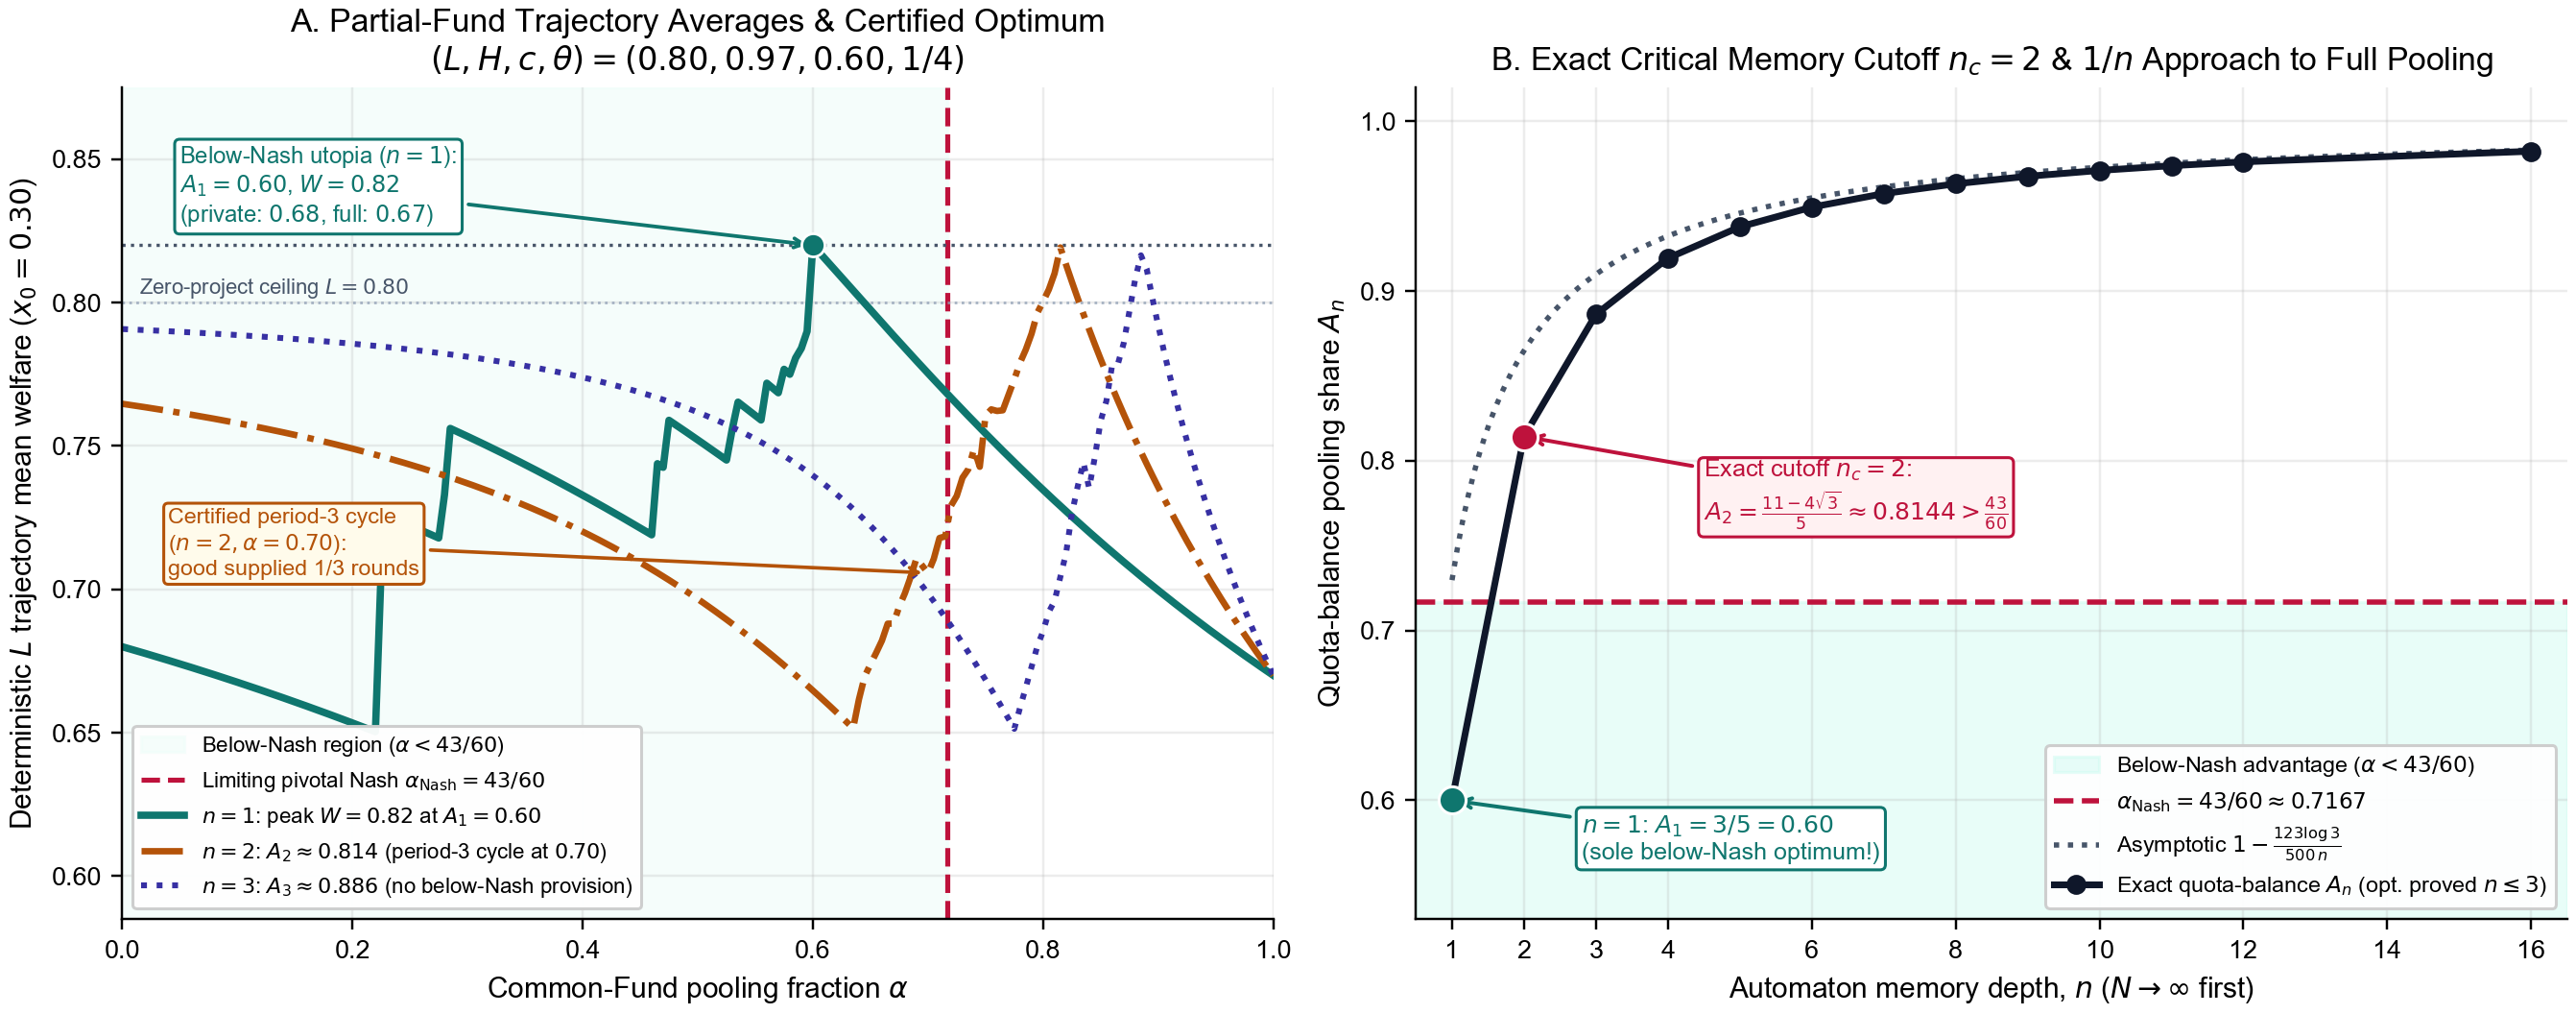
\includegraphics[width=\textwidth]{figs/p2_fig3_common_fund_cutoff.png}
  \caption{\textbf{Partial Common Fund trajectory averages and the exact $n_c = 2$ memory cutoff.}
  \textbf{(A)} Binary64 deterministic $L$ mean-field trajectory averages ($x_0 = 0.30$, 800 burn-in, 120 averaging steps) across $\alpha \in [0,1]$ in $(0.80,0.97,0.60,1/4)$, overlaid with independently proved benchmarks: depth-$1$ optimum $W = 0.82$ at $A_1 = 0.60 < \alpha_{\mathrm{Nash}} = 43/60$ (vs.\ private $0.68$ and full $0.67$), and the certified period-$3$ limit cycle at $(n=2, \alpha=0.70)$.
  \textbf{(B)} Exact quota-balance shares $A_n$ vs.\ memory depth $n$: crossing $\alpha_{\mathrm{Nash}}$ at $n_c = 2$ ($A_2 = \frac{11-4\sqrt{3}}{5} \approx 0.8144$) and approaching $100\%$ as $1 - \frac{123\log 3}{500\,n}$.}
  \label{fig:p2-fund}
\end{figure}

\section{Formal Machine Verification and Honest Open Problems}\label{sec:lean}

Core algebraic pillars of Theorems~\ref{thm:memory-cliffs}, \ref{thm:staghunt}, \ref{thm:fund-n1}, and \ref{thm:fund-cutoff} are formally verified in standalone Lean~4.36.0 under \texttt{proofs/lean4/} in the modules \texttt{EscapeGeometry} (25 public theorems: $N$-player public-good cutoff $d_* = h(N-2)/(N-1)$ and exact $(1,1)\to(2,1)$ stationary memory-upgrade witness), \texttt{StagHuntMirage} (23 public theorems: reference flux \eqref{eq:ref-flux}, ladder cancellation \eqref{eq:ladder-cancel}, critical curve equivalence, unique 4-state depth-$1$ stationary law with $\pi_1(CC)=1300/3517$ at $(47/50,4/5,1/2)$, and all three rational upper-corner bounds $<3/8$), and \texttt{CommonFundCutoff} (40 public theorems: exact depth-$1$ quota-balance equation and feasibility, strict monotonicity of $R_n$, exact $n_c = 2$ cutoff $123/55 < 3 < (123/55)^2$, exact quadratic $25 A_2^2 - 110 A_2 + 73 = 0$ with bracket $814/1000 < A_2 < 815/1000$, exclusion of every productive fixed point at $\alpha \le 43/60$, and a uniform depth-$2$ stationary welfare gap $\ge 3027/1600000$ derived from the stationarity bridge), within a 5-module suite totaling 117 public theorems (60 private lemmas), zero \texttt{sorry}, and only standard Lean axioms audited across all 911 theorem constants (out of 1,168 declarations). Analytical large-$N$ optimizer convergence supplements the Lean quota identities. Numerical certificates are documented per dataset: exact rational payoff enclosures of width $4.0\times 10^{-70}$ at $(40,40)$ and $1.76\times 10^{-66}$ at $(41,40)$, 76 certified digits (up to 434-digit working precision) across 368 Stag Hunt solves, and 80-digit interval contraction boxes for the $(n=2, \alpha=0.70)$ period-$3$ cycles (\texttt{experiments/phase1\_memory.py}, \texttt{phase2b\_staghunt\_robustness.py}, \texttt{phase2b\_quorum\_memory.py}).

\subsection*{Open Problems}
Four crisp analytical questions remain open:
\begin{enumerate}
  \item \emph{Critical Stag-Hunt leading constant for fixed $S < 1/2$}: Theorem~\ref{thm:staghunt}(1) proves $U_n = \Theta(1)$ at $R = R_c(P,S)$ for fixed $S < 1/2$ and gives $K$ for $S \ge 1/2$ (and uniformly as $S \to 1/2$); determining the exact limiting constant for fixed $S < 1/2$ remains open.
  \item \emph{Global attraction of the $(n=2, \alpha=0.70)$ period-$3$ limit cycles}: While we certify existence and strict local contraction ($< 18/25$ for $L$, $< 17/20$ for $B$) on radius-$10^{-80}$ return-map boxes, ruling out other attractors across the entire $3$-dimensional probability simplex remains open.
  \item \emph{Finite-$N$ global maximizer convergence at depth $n \ge 4$ and critical rate at $A_3$}: In Theorem~\ref{thm:fund-cutoff}, the quota-balance shares $A_n$ and $1-A_n \sim C/n$ hold for all feasible depths, and actual convergence $\alpha_{N,n}^{\mathrm{opt}} \to A_n$ is proved for $n \in \{1, 2, 3\}$; extending global maximizer selection to $n \ge 4$ (and determining the exact finite-$N$ deficit rate at $A_3$) remains open.
  \item \emph{Independent-signal $N$-player public-good cutoff}: Extending Theorem~\ref{thm:memory-cliffs}(3) from action-group-shared signals to independent individual feedback and simultaneous fixed-ratio limits $m/n \to \gamma$ remains open.
\end{enumerate}

\begin{thebibliography}{99}
\bibitem{Tsetlin1961}
M.~L.~Tsetlin, \emph{On the behavior of finite automata in random media}, Avtomat.\ i Telemekh.\ \textbf{22}:10 (1961), 1345--1354 (Russian; Math-Net.Ru \texttt{at12417}).

\bibitem{Tsetlin1963}
M.~L.~Tsetlin, \emph{Finite automata and models of simple forms of behavior}, Uspekhi Mat.\ Nauk \textbf{18}:4(112) (1963), 3--28 (Russian; Math-Net.Ru \texttt{rm6373}).

\bibitem{GPST1963}
I.~M.~Gelfand, I.~I.~Pyatetskii-Shapiro, and M.~L.~Tsetlin, \emph{On certain classes of games and automata games}, Dokl.\ Akad.\ Nauk SSSR \textbf{152}:4 (1963), 845--848 (Russian; Math-Net.Ru \texttt{dan28648}).

\bibitem{GKT1964}
S.~L.~Ginzburg, V.~Yu.~Krylov, and M.~L.~Tsetlin, \emph{One example of a game of many identical automata}, Avtomat.\ i Telemekh.\ \textbf{25}:5 (1964), 668--672 (Russian; Math-Net.Ru \texttt{at11654}).

\bibitem{Pittel1965}
B.~G.~Pittel, \emph{On asymptotic properties of one variant of the Gur game}, Probl.\ Peredachi Inf.\ \textbf{1}:3 (1965), 99--112 (Russian; Math-Net.Ru \texttt{ppi752}).

\bibitem{Krinskii1966}
V.~I.~Krinskii, \emph{Zero-sum games for two asymptotically optimal sequences of automata}, Probl.\ Peredachi Inf.\ \textbf{2}:2 (1966), 43--53 (Russian; English transl.\ \textbf{2}:2 (1966), 33--41; Math-Net.Ru \texttt{ppi1933}).

\bibitem{PalfreyRosenthal1984}
T.~R.~Palfrey and H.~Rosenthal, \emph{Participation and the provision of discrete public goods: a strategic analysis}, J.\ Public Econ.\ \textbf{24}:2 (1984), 171--193.

\bibitem{Paper1}
Project ReMath, \emph{Shared Fate and Imperfect Synchrony in Tsetlin's Collective Automata: Architecture Hierarchies, Unequal-Memory Optimal Correlation, and Two-Dimensional Escape Geometry}, companion preprint, Study~\#02 (2026).
\end{thebibliography}

\end{document}
